\documentclass[11pt,a4paper]{article}

\usepackage{epsfig}
\usepackage{multicol}

\usepackage[utf8]{inputenc}
\usepackage[brazil]{babel}
\usepackage{fancyheadings}
\usepackage{amsmath}
\usepackage{calrsfs}
\usepackage{enumerate}
\DeclareGraphicsExtensions{.png,.pdf}
\usepackage{amsmath, amsfonts, amssymb}
\usepackage{esint}
\usepackage{graphicx}
\usepackage{multicol}
\usepackage{tasks}
\usepackage[utf8]{inputenc}
\usepackage{mathrsfs} % Transformada de Laplace
\usepackage{indentfirst}

% As margens
\setlength{\textheight}{24.0cm}
\setlength{\textwidth}{17.5cm}
\setlength{\oddsidemargin}{2.0cm} % Margens reais desejadas
\setlength{\evensidemargin}{2.0cm} % 2+17.5+1.5=21cm (largura A4)
\setlength{\topmargin}{1.5cm} % 1.5+1.6+1.0+24.0+1.6=29.7cm
\setlength{\headheight}{1.6cm} % (altura A4)
\setlength{\headsep}{1.0cm}
\setlength{\columnsep}{1.5cm} % Coluna = 8cm ((17.5-1.5)/2)
\addtolength{\oddsidemargin}{-1in}
\addtolength{\evensidemargin}{-1in}
\addtolength{\topmargin}{-1in}
\setlength{\footskip}{0.0cm}


% Novos comandos
\newcommand{\limite}{\displaystyle\lim}
\newcommand{\integral}{\displaystyle\int}
\newcommand{\somatorio}{\displaystyle\sum}
\newcommand{\mat}[1]{\mbox{\boldmath{$#1$}}} 

\pagestyle{fancy}


\usepackage{lipsum}

\lhead{

\includegraphics[width=1cm]{brasao.png}
}

\rhead{ 
\sc\textbf{U}niversidade \textbf{F}ederal do \textbf{C}eará\\
Campus Quixadá\\ Monitoria de Cálculo II, III e EDO}

\cfoot{}

\begin{document}

	\begin{center}
		\Large Lista 5 - Integrais de Linha e Campos Conservativos
	\end{center}
	

	\begin{enumerate}
	
	\item Calcule $\displaystyle\int_\gamma \vec{F} \cdot d\vec{r}$ sendo dados:
	
	\begin{enumerate}
	\item $\vec{F}(x,y,z) = x\vec{i} + y\vec{j} + z\vec{k}$ e $\gamma (t) = (\cos t \textrm{,}\ \sin t \textrm{,}\ t)$, $0 \leq t \leq 2\pi$.
	\item $\vec{F}(x,y,z) = (x + y + z)\vec{k}$ e $\gamma (t) = (t \textrm{,}\ t \textrm{,}\ 1 - t^2)$, $0 \leq t \leq 1$.
	\item $\vec{F}(x,y) = x^2\vec{j}$ e $\gamma (t) = (t^2 \textrm{,}\ 3)$, $-1 \leq t \leq 1$.
	\item $\vec{F}(x,y) = x^2\vec{i} + (x - y)\vec{j}$ e $\gamma (t) = (t \textrm{,}\ \sin t \textrm{,}\ t)$, $0 \leq t \leq \pi$.
	\item $\vec{F}(x,y,z) = x^2\vec{i} + y^2\vec{j} + z^2\vec{k}$ e $\gamma (t) = (2\cos t \textrm{,}\ 3\sin t \textrm{,}\ t)$, $0 \leq t \leq 2\pi$.
	
	\end{enumerate}

\item Uma partícula move-se no plano de modo que no instante $t$ sua posição é dada por $\gamma (t) = (t \textrm{,}\ t^2)$. Calcule o trabalho realizado pelo campo de forças $\vec{F}(x,y) = (x + y)\vec{i} + (x - y)\vec{j}$ no deslocamento da partícula de $\gamma (0)$ até $\gamma (1)$.

\item Uma partícula desloca-se em um campo de forças dado por $\vec{F}(x,y,z) = -y\vec{i} + x\vec{j} + z\vec{k}$. Calcule o trabalho realizado por $\vec{F}$ no deslocamento da partícula de $\gamma (a)$ até $\gamma (b)$, sendo dados

\begin{enumerate}

\item $\gamma (t) = (\cos t \textrm{,}\ \sin t \textrm{,}\ t)$, $a = 0$ e $b = 2 \pi$.
\item $\gamma (t) = (2t + 1 \textrm{,}\ t - 1 \textrm{,}\ t)$, $a = 1$ e $b = 2 $.
\item $\gamma (t) = (\cos t \textrm{,}\ 0 \textrm{,}\ \sin t)$, $a = 0$ e $b = 2 \pi$.

\end{enumerate}

\item Calcule $\displaystyle\int_\gamma \vec{E} \cdot d\vec{l}$ onde $\vec{E}(x,y) = \dfrac{1}{x^2 + y^2} \dfrac{x \vec{i} + y \vec{j}}{\sqrt{x^2 + y^2}}$ e $\gamma (t) = (t \textrm{,}\ 1)$, $-1 \leq t \leq 1$. (O $\vec{l}$ desempenha aqui o mesmo papel que o $\vec{r}:\vec{l}(t) = \gamma (t)$.)

\item Seja $\vec{E}$ o campo do exercício anterior e seja $\gamma$ a curva dada por $x = t$ e $y = 1 - t^4$,  $-1 \leq t \leq 1$.
\begin{enumerate}
\item Que valor é razoável esperar para $\displaystyle\int_\gamma \vec{E} \cdot d\vec{l}$? Por quê?
\item Calcule $\displaystyle\int_\gamma \vec{E} \cdot d\vec{l}$.
\end{enumerate}

\item Calcule $\displaystyle\int_\gamma \vec{E} \cdot d\vec{l}$ onde $\vec{E}$ é o campo dado no exercício 4 e $\gamma$ a curva dada por $x = 2\cos t$, $y = \sin t$ com $0 \leq t \leq \pi/2$.

\item Calcule $\displaystyle\int_\gamma x \ dx + y \ dy$, sendo $\gamma$ dada por $x = r^2$ e $y = \sin t$, $0 \leq t \leq \pi/2$.

\item Calcule $\displaystyle\int_\gamma x \ dx - y \ dy$, onde $\gamma$ é o segmento de extremidades $(1 \textrm{,}\ 1)$ e $(2 \textrm{,}\ 3)$, percorrido no sentido de $(1 \textrm{,}\ 1)$ para $(2 \textrm{,}\ 3)$.

\item Calcule $\displaystyle\int_\gamma x \ dx + y \ dy + z \ dz$, onde $\gamma$ é o segmento de extremidades $(0 \textrm{,}\ 0 \textrm{,}\ 0)$ e $(1 \textrm{,}\ 2 \textrm{,}\ 1)$, percorrido no sentido de $(1 \textrm{,}\ 2 \textrm{,}\ 1)$ para $(0 \textrm{,}\ 0 \textrm{,}\ 0)$.

\item Calcule $\displaystyle\int_\gamma x \ dx + dy + 2 \ dz$ onde $\gamma$ é a interseção do parabolóide $z = x^2 + y^2$ com o plano $z = 2x + 2y - 1$; o sentido de percurso deve ser escolhido de modo que a projeção de $\gamma (t)$, no plano $xy$, caminhe no sentido anti-horário.

\item Calcule $\displaystyle\int_\gamma \ dx + xy \ dy + z \ dz$, onde $\gamma$ é a interseção de $x^2 + y^2 + z^2 = 2$, $x \geq 0$, $y \geq 0$ e $z \geq 0$, com o plano $y = x$; o sentido de percurso é do ponto $(0 \textrm{,}\ 0 \textrm{,}\ \sqrt{2})$ para $(1 \textrm{,}\ 1 \textrm{,}\ 0)$.

\item Calcule $\displaystyle\int_\gamma 2 \ dx - dy$, onde $\gamma$ tem por imagem $x^2 + y^2 = 4$, $x \geq 0$ e $y \geq 0$; o sentido de percurso é de $(2 \textrm{,}\ 0)$ para $(0 \textrm{,}\ 2)$.

\item Calcule $\displaystyle\int_\gamma \dfrac{-y}{4x^2 + y^2} \ dx + \dfrac{x}{4x^2 + y^2} \ dy$, onde $\gamma$ tem por imagem a elipse $4x^2 + y^2 = 9$ e o sentido de percurso é o anti-horário.

\item Seja $\gamma(t) = (R\cos t \textrm{,}\ R\sin t)$, $0 \leq t \leq 2\pi$ com $(R > 0)$. Mostre que $\displaystyle\int_\gamma \dfrac{-y}{4x^2 + y^2} \ dx + \dfrac{x}{4x^2 + y^2} \ dy$ não depende de $R$.

\item Calcule $\displaystyle\int_\gamma dx + y \ dy + dz$ onde $\gamma$ é a interseção do plano $y = x$ com a superfície $z = x^2 + y^2$, $z \leq 2$, sendo o sentido de percurso do ponto $(-1 \textrm{,}\ -1 \textrm{,}\ 2)$ para o ponto $(0 \textrm{,}\ 0 \textrm{,}\ 2)$.

\item Calcule $\displaystyle\int_\gamma dx +  dy + dz$ onde $\gamma$ é a interseção entre as superfícies $y = x^2$ e $z = 2 - x^2 - y^2$, $x \geq 0$, $y \geq 0$ e $z \geq 0$, sendo o sentido de percurso do ponto $(1 \textrm{,}\ 1 \textrm{,}\ 0)$ para o ponto $(0 \textrm{,}\ 0 \textrm{,}\ 2)$.

\item Calcule $\displaystyle\int_\gamma 2y \ dx +  z \ dy + x \ dz$ onde $\gamma$ é a interseção das superfícies $x^2 + 4y^2 = 1$ e $x^2 + z^2 = 1$, $y \geq 0$ e $z \geq 0$ sendo o sentido de percurso do ponto $(1 \textrm{,}\ 0 \textrm{,}\ 0)$ para o ponto $(-1 \textrm{,}\ 0 \textrm{,}\ 0)$.

\item Calcule $\displaystyle\int_\gamma \sqrt[3]{x} \ dx + \dfrac{dy}{1 + y^2}$, onde $\gamma$ é a curva

\begin{figure}[h]	
\centering % para centralizarmos a figura	
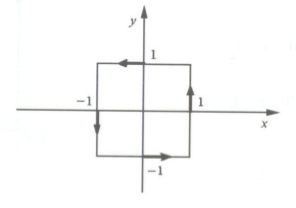
\includegraphics[width=5cm]{Selection_029.jpg} 
\end{figure}

\item Calcule $\displaystyle\int_\gamma \vec{F} \cdot d\vec{r}$, onde $\vec{F}(x,y) = (x + y)\vec{j}$ e $\gamma$ é a curva do exercício anterior. 

\item Calcule $\displaystyle\int_\gamma (x - y) \ dx + e^{x + y} \ dy$, onde $\gamma$ é a fronteira do triângulo de vértices $(0 \textrm{,}\ 0)$, $(0 \textrm{,}\ 1)$ e $(1 \textrm{,}\ 2)$. orientada no sentido anti-horário.

\item Calcule $\displaystyle\int_\gamma y^2 \ dx + x \ dy - dz$, onde $\gamma$ é a poligonal de vértices $A_0 = (0 \textrm{,}\ 0 \textrm{,}\ 0)$, $A_1 = (1 \textrm{,}\ 1 \textrm{,}\ 1)$ e $A_2 = (1 \textrm{,}\ 1 \textrm{,}\ 0)$, orientada de $A_0$ para $A_2$. 

\item Calcule $\displaystyle\int_\gamma x^2 \ dx + y^2 \ dy + z^2 \ dz$ onde $\gamma$ é a curva do exercício anterior.

\item Verifique que 
$$\displaystyle\int_\gamma P \ dx + Q \ dy = \displaystyle\iint_B \left(\dfrac{\partial Q}{\partial x} - \dfrac{\partial P}{\partial y}\right) dx \ dy $$

onde $P$ e $Q$ são supostas de classe $C^1$ num aberto $\Omega$ contendo $B$.

(Sugestão: Calcule $\displaystyle\iint_B \dfrac{\partial Q}{\partial x} \ dx \ dy$  fixando, inicialmente, $y$; calcule $- \displaystyle\iint_B \dfrac{\partial P}{\partial y} \ dx \ dy$ fixando, inicialmente, $x$. Compare, em seguida, com as integrais $\displaystyle\int_\gamma Q \ dy$ e $\displaystyle\int_\gamma P \ dx$.)

\item Verifique a relação do exercício anterior supondo $B$ o quadrado de vértices $(-1 \textrm{,}\ -1)$, $(1 \textrm{,}\ -1)$, $(1 \textrm{,}\ 1)$ e $(-1 \textrm{,}\ 1)$; $\gamma$ a fronteira de $B$ orientada no sentido anti-horário.

\item Sejam $f, g:[a,b] \to \mathbb{R}$ duas funções de classe $C^1$ tais que, para todo $x$ em $[a,b]$, $f(x) < g(x)$. Seja $B$ o conjunto de todos $(x,y)$ tais que $f(x) \leq y \leq g(x)$, $a \leq x \leq b$. Seja $\gamma$ a fronteira de $B$ orientada no sentido anti-horário. Prove que
$$\displaystyle\int_\gamma P \ dx = \displaystyle\iint_B - \dfrac{\partial P}{\partial y} \ dx \ dy$$
onde $P$ é suposta de classe $C^1$ num aberto que contém $B$.

\item Sejam $B$ e $\gamma$ como no exercício anterior. Prove que
$$\textrm{área de B} = - \displaystyle\int_\gamma y \ dx $$.

\item Calcule a massa do fio $\gamma (t) = (t \textrm{,}\ 2t \textrm{,}\ 3t)$, $0 \leq t \leq 1$, cuja densidade linear é $\delta (x,y,z) = x + y + z$.

\item Calcule a massa do fio $\gamma (t) = (\cos t \textrm{,}\ \sin t \textrm{,}\ t)$, $0 \leq t \leq \pi$, cuja densidade linear é $\delta (x,y,z) = x^2 + y^2 + z^2$.

\item Calcule o momento de inércia de um fio homogêneo com a forma de uma circunferência de raio $R$, em torno de um diâmetro. 

\item Calcule o momento de inércia do fio $\gamma (t) = (t \textrm{,}\ 2t \textrm{,}\ 3t)$, $0 \leq t \leq 1$, com densidade linear $\delta (x,y,z) = x + y + z$ em torno do eixo $O_z$.

\item Calcule o momento de inércia de um fio retilíneo, homogêneo, de comprimento L, em torno de um eixo perpendicular ao fio e passando por uma das extremidades do fio. 

\item O centro de massa de um fio $\gamma:[a,b] \to \mathbb{R}^3$ é o ponto $(x_c, y_c, z_c)$ dado por:

$$x_c = \displaystyle\dfrac{\displaystyle\int_\gamma x \ dm}{\displaystyle\int_\gamma dm} \textrm{,}\ y_c = \displaystyle\dfrac{\displaystyle\int_\gamma y \ dm}{\displaystyle\int_\gamma dm} \textrm{ e}\ z_c = \displaystyle\dfrac{\displaystyle\int_\gamma z \ dm}{\displaystyle\int_\gamma dm}$$

onde $dm = \delta(x,y,z) \ ds$ é o elemento de massa. Calcule o centro de massa do fio homogêneop dado

\begin{enumerate}
\item $\gamma (t) = (\cos t \textrm{,}\ \sin t \textrm{,}\ t)$, $0 \leq t \leq \pi/2 $.
\item $\gamma (t) = (t \textrm{,}\ t^2 \textrm{,}\ 0)$, $-1 \leq t \leq 1$.
\end{enumerate} 

\item Experiências mostram que uma corrente contínua $I$ em um fio comprido produz um campo magnético $B$ que é tangente a qualquer círculo em um plano perpendicular ao fio cujo centro seja o eixo do fio (como na figura). A Lei de Ampère relaciona a corrente elétrica ao campo magnético criado e afirma que
$$\displaystyle\int_ C \vec{B} \cdot d\vec{r} = \mu_0 I$$

onde $I$ é a corrente total que passa por qualquer superfície limitada por uma curva fechada $C$, e $\mu_0$ é uma constante chamada permeabilidade no vácuo. Tomando $C$ como um círculo de raio r, mostre que o módulo $B = |B|$ do campo magnético a uma distância $r$ do centro do fio é dado por
$$B = \displaystyle\dfrac{\mu_0 I}{2\pi r}$$

\begin{figure}[h]	
\centering % para centralizarmos a figura	
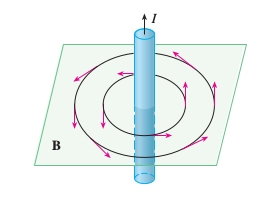
\includegraphics[width=5cm]{Selection_030.jpg} 
\end{figure}

\item Verifique se o campo vetorial

$$\vec{V} = (2y \cos z - 3y^2)\mat{\hat{i}} + (2x\cos z - 6xy)\mat{\hat{j}} + (4\cos z - 2xy \sin z)\mat{\hat{k}}$$

é conservativo. Se for, obtenha a função $f$ tal que $\vec{V} = \nabla f$.

\item Considerando que uma força dada por
$$\vec{F} = (3xy - z)\mat{\hat{i}} + 2x^2\mat{\hat{j}} - 3xz\mat{\hat{k}}$$
aja sobre uma partícula de massa $m$, determine o trabalho realizado pela força para levar a partícula do ponto $A(1 \textrm{,}\ -2 \textrm{,}\ 1)$ ao ponto $B(3 \textrm{,}\ 1 \textrm{,}\ 4)$ ao longo da trajetória descrita pela equação
$$r(\vec{t}) = (t + 1)\mat{\hat{i}} + \left(\dfrac{3t^2}{8} - 2 \right)\mat{\hat{j}} + \left[(t + 1)^2 - \dfrac{5t}{2} \right]\mat{\hat{k}}$$
onde $t$ é o tempo, e as unidades utilizadas são do $SI$.

\item Verifique se a força

$$\vec{F} = -15x^4y\mat{\hat{i}} + (2z^2 - 3x^5)\mat{\hat{j}} + 4yz\mat{\hat{k}}$$

é conservativa e, em caso positivo, ache o trabalho realizado para ir do ponto inicial $A(1 \textrm{,}\ 2 \textrm{,}\ -1)$ ao ponto final $B(0 \textrm{,}\ 1 \textrm{,}\ 1)$. Todas as unidades são do SI.

\item A força gravitacional exercida pela Terra sobre um objeto de massa $m$ situado em suas proximidades pode ser escrita como 
$$\vec{F} = - mg \mat{\hat{k}}$$
onde o eixo $z$ aponta na direção da vertical de prumo no local, com sentido para cima, e $g$ é o módulo da aceleração da gravidade no local. Verifique se essa força é conservativa. Caso seja, encontre a energia potencial associada.

\item A força gravitacional exercida por uma partícula de massa $m_1$ sobre uma partícula de massa $m_2$ situada a uma distância $r$ de $m_1$ é conservativa, e ela é dada por
$$\vec{F} = - \displaystyle\dfrac{G m_1 m_2}{r^2} \mat{\hat{r}}$$

onde $G$ é a constante de gravitação universal e $\mat{\hat{r}}$ é um versor orientado de $m_1$ para $m_2$. Obtenha a energia potencial associada.

\item Considere a força eletrostática produzida por uma carga pontual $Q$ sobre uma carga $q$ também pontual, estando ambas situadas no vácuo, a qual é dada, no SI, pela expressão
$$\vec{F}_{Q \to q} = \displaystyle\dfrac{1}{4\pi \epsilon_0}\displaystyle\dfrac{qQ}{r^2}\mat{\hat{r}}$$
Determine a energia potencial elétrica $U$ associada a essa força.

\item O campo elétrico produzido por um fio retilíneo muito longo e fino imerso em vácuo e contendo cargas distribuídas de forma homogênea ao longo de seu comprimento é dado por

$$\vec{E} = \displaystyle\dfrac{\lambda}{2\pi \varepsilon_0 \rho}\mat{\hat{\rho}}$$
onde $\lambda$ é a densidade linear de cargas no fio. Determine o potencial elétrico correspondente.

\item Uma esfera de raio R contém cargas distribuídas em seu interior de forma que a densidade volumétrica de carga correspondente vale

$$\varrho(r) = kr \textrm{,}\ r \leq R$$

onde $k$ é uma constante e $r$ é a distância de um ponto da esfera ao seu centro. O campo elétrico gerado por essa esfera é dado por

$$\vec{E}(\vec{r}) = 
		\begin{cases}
			\displaystyle\dfrac{kr^2}{4\varepsilon_0}\, \quad\quad r \leq R \\
			\displaystyle\dfrac{kR^4}{4\varepsilon_0 r^2}\, \quad r \geq R \\
		\end{cases}
	$$
	
onde $r$ é a distância de um ponto qualquer do espaço até o centro da esfera. Determine o potencial elétrico correspondente nas duas regiões. Considere, como ponto de referência, a superfície da esfera, que está sujeita a um potencial $V(R) = V_0$.
 
\end{enumerate}		
	
\end{document}